\documentclass{physlab}

\begin{document}
\begin{titlepage}
\center % Center everything on the page
 
%----------------------------------------------------------------------------------------
%	HEADING SECTIONS
%----------------------------------------------------------------------------------------

\textsc{\LARGE Московский\\[-0.2cm]Физико-Технический Институт\\[0.1cm]\large (государственный университет)}\\[1.5cm] % Name of your university/college
\textsc{\Large Кафедра общей физики}\\[0.1cm] % Major heading such as course name
\textsc{\large Лабораторная работа № 1.2}\\[0.5cm] % Minor heading such as course title

%----------------------------------------------------------------------------------------
%	TITLE SECTION
%----------------------------------------------------------------------------------------

\HRule
\\[0.6cm]
{\huge \bfseries Эффект Комптона}
\\[0.3cm] % Title of your document
\HRule
\\[1.5cm]


 
%----------------------------------------------------------------------------------------
%	AUTHOR SECTION
%----------------------------------------------------------------------------------------

\begin{minipage}[t]{0.48\textwidth}
	\begin{flushleft} \large
		\textsf{Студент}
		
		Ришат \textsc{Исхаков} \\[-0.15cm]
		512 группа

	\end{flushleft}
\end{minipage}
\hfill
\begin{minipage}[t]{0.48\textwidth}
	\begin{flushright} \large
		\textsf{Преподаватель}		
		
		Лев Владиславович \\[-0.15cm]
		\textsc{Инжечик} 

	\end{flushright}
\end{minipage}

\begin{bottompar}
	\begin{center}
		\includegraphics[width = 80 mm]{logo.jpg}
	\end{center}
	\today

\end{bottompar}
\vfill % Fill the rest of the page with whitespace

\end{titlepage}

\paragraph{Цель работы:} Методом электронного возбуждения измерить энергию первого уровня атома гелия в динамическом и статическом режимах.

\section{Теория}
Опыт Франка-Герца -- это один из простейших экспериментов, доказывающих существование дискретных уровней энергии атомов.

\begin{wrapfigure}{R}{0.5\linewidth}
\centering
    \includegraphics[width=.7\linewidth]{1.png}
\caption{Принципиальная схема опыта}
\label{scheme} 
\end{wrapfigure}

Разреженный одноатомный газ заполняет трехэлектродную лампу(рис. \ref{scheme}).  Электроны, испускаемые разогретым катодом, ускоряются в постоянном электрическом поле, созданным между катодом и сетчатым анодом лампы. Передвигаясь от катода к аноду, электроны сталкиваются с атомами гелия. Если энергия электрона, налетающего на атом, недостаточна для того, чтобы перевести его в возбужденное состояние, то возможны только упругие столкновения, при которых электроны почти не теряют энергии, так как их масса в тысячи раз меньше массы атомов. 


По мере увеличения разности потенциалов между анодом и катодом энергия электронов увеличивается и, в конце концов, оказывается достаточной для возбуждения атомов. При таких -- неупругих -- столкновениях кинетическая энергия налетающего электрона передается одному из атомных электронов, вызывая его переход на свободный энергетический уровень (возбуждение) или совсем отрывая его от атома (ионизация).

\begin{wrapfigure}[12]{L}{0.5\linewidth} 
\centering
    \includegraphics[width=.7\linewidth]{2.png}
\caption{Зависимость тока коллектора от напряжения на аноде}
\label{dependency}
\end{wrapfigure}

Третьим электродом лампы является коллектор. Между ним и анодом поддерживается небольшое задерживающее напряжение (потенциал коллектора меньше потенциала анода). Ток коллектора, пропорциональный числу попадающих на него за секунду электронов, измеряется микроамперметром.


При увеличении потенциала анода ток в лампе вначале растет, подобно тому как это происходит в вакуумном диоде(рис. \ref{dependency}). Однако, когда энергия электронов становится достаточной для возбуждения атомов, ток коллектора резко уменьшается. Это происходит потому, что при неупругих соударениях с атомами электроны почти полностью теряют свою энергию и не могут преодолеть задерживающего потенциала между анодом и коллектором. При дальнейшем увеличении потенциала анода ток коллектора вновь возрастает: электроны, испытавшие неупругие соударения, при дальнейшем движении к аноду успевают набрать энергию, достаточную для преодоления задерживающего потенциала. Следующее замедление роста тока происходит в момент, когда часть электронов неупрого сталкивается с атомами два раза: первый раз посередине пути, второй -- у анода и т.д. Таким образом, на кривой зависимости тока коллектора от напряжения анода имеется ряд максимумов и минимумов, отстоящих друг от друга на равные расстояния $\Delta V$.

\section{Экспериментальная установка}

\begin{wrapfigure}{r}{0.5\linewidth} \label{fullscheme} 
\vspace{-5ex}  
 \center{\includegraphics[width=.7\linewidth]{3.png}}
\caption{Схема установки}
\end{wrapfigure}


Для опыта используется лампа ионизационного манометра ЛМ-2, заполненная гелием до давления $\sim 1$ Торр. Напряжение накала подается от источника питания C. Ток накала контролируется амперметром А. Ускоряющее напряжение подается на анод от выпрямителя B. Ток в цепи коллектора регистрируется микроамперметром.

Схему можно переключать из статического режима измерений в динамический. При нем ускоряющий потенциал подается с понижающего трансформатора Т( 220/50 В), а ток коллектора регистрируется осциллографиом, подключенным к нагрузочному резистору R. 


\section{Обработка полученных результатов}

\subsection{Динамический режим}

\begin{figure}[H]
    \centering
    \begin{subfigure}[b]{0.3\textwidth}
        \includegraphics[width=\textwidth]{4V}
        \caption{$4 \; \V$}
        \label{fig:actuatorscouplingSheme_decoupledcase}
    \end{subfigure}
    ~ %add desired spacing between images, e. g. ~, \quad, \qquad, \hfill etc. 
      %(or a blank line to force the subfigure onto a new line)
    \begin{subfigure}[b]{0.3\textwidth}
        \includegraphics[width=\textwidth]{6V}
        \caption{$6 \; \V$}
        \label{fig:actuatorscouplingSheme_nearestcoupledcase}
    \end{subfigure}
    ~ %add desired spacing between images, e. g. ~, \quad, \qquad, \hfill etc. 
    %(or a blank line to force the subfigure onto a new line)
    \begin{subfigure}[b]{0.3\textwidth}
        \includegraphics[width=\textwidth]{8V}
        \caption{$8 \; \V$}
        \label{fig:actuatorscouplingSheme_nearestcoupled_and_diag_case}
    \end{subfigure}
    \caption{Зависимость тока коллектора от напряжения на аноде в динамическом режиме при различных запирающих напряжениях}
    \label{fig:threeDMcases}
\end{figure}


\begin{table}[H]
\centering
\begin{tabular}{|c|c|c|c|}
\hline
Запирающее напряжение& $4 \; \V$      & $6 \; \V$      & $8 \; \V$      \\ \hline
$\Delta V_{max}, \; \V$ & $19 $ & $ 20 $& $ 20 $\\ \hline
$\Delta V_{min}, \; \V$ & $18 $ & $ 17 $& $ 18 $\\ \hline
\end{tabular}
\caption{Измеренные значения в динамическом режиме}
\end{table}

Получаем:
\[E_1 = e \overline{\Delta V_{max}} = 19.7 \; \eV \]
\[\sigma_{\Delta V} = 0.57 \; \eV \]

\subsection{Статический режим}
\begin{figure}[H]
    \center{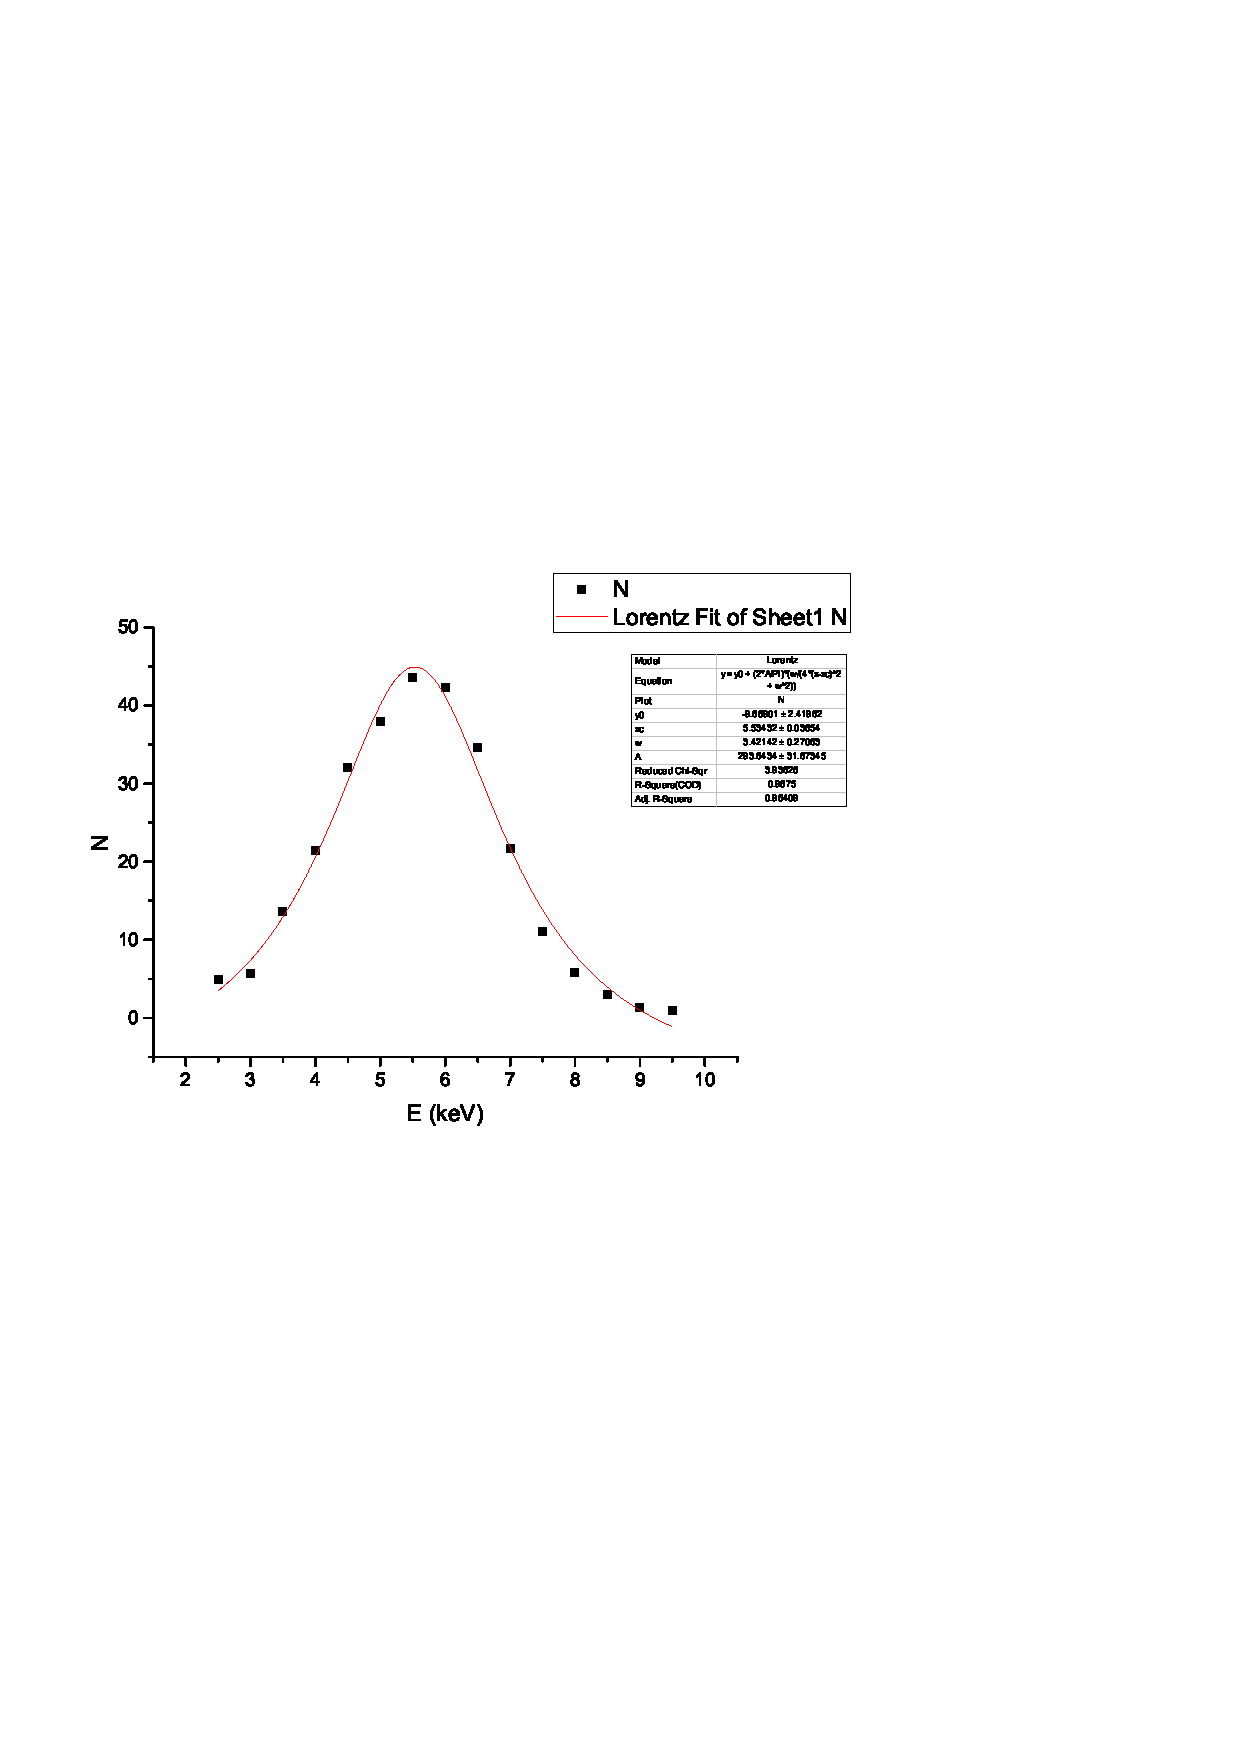
\includegraphics[width=\linewidth]{graph.pdf}}
\caption{Семейство зависимостей тока коллектора от напряжения на аноде}
\end{figure}

По данным графиков:

\begin{table}[h]
\centering
\begin{tabular}{|c|c|c|c|}
\hline
Запирающее напряжение & $4 \; \V$      & $6 \; \V$      & $8 \; \V$      \\ \hline
$\Delta V_{max}, \; \V$ & $19.21$ & $19.40$& $19.91$\\ \hline
$\Delta V_{min}, \; \V$ & $21.12$ & $22.74$& $20.40$\\ \hline
\end{tabular}
\caption{Измеренные значения в статическом режиме}
\end{table}

Получаем:
\[E_1 = e \overline{\Delta V_{max}} = 19.51 \; \eV \]
\[\sigma_{\Delta V} = 0.36 \; \eV \]

\section{Вывод}
В ходе опыта была прослежена дискретная природа энергитических уровней атома гелия. Были получены значения первого энергетического уровня атома гелия в динамическом ($19.70 \pm 0.57 \; \eV$) и статическом ($19.51 \pm 0.36 \; \eV$) режимах. Полученные результаты совпадают с табличным значением ($19.82 \; \eV$) с точностью до погрешности.

\end{document}